\documentclass[]{article}
\usepackage{amsmath}
\usepackage{amsfonts}
\usepackage{amssymb}
\usepackage{tikz}
\usepackage{graphicx}
\usepackage{listings}

\definecolor{dkgreen}{rgb}{0,0.6,0}
\definecolor{gray}{rgb}{0.5,0.5,0.5}

\lstset{
  language=Python,
  breaklines=true,
  showstringspaces=false,
  frame=single,
  aboveskip=3mm,
  belowskip=3mm,
  columns=flexible,
  basicstyle={\small\ttfamily},
  numbers=none,
  numberstyle=\tiny\color{gray},
  keywordstyle=\color{blue},
  commentstyle=\color{gray},
  stringstyle=\color{dkgreen},
  breakatwhitespace=true,
  tabsize=3
}

\title{CAGD - Homework 6}
\author{Josefine St{\aa}l \& Erik Ackzell}

\begin{document}

\maketitle
\section*{Task 1}
In this task we plot a 3D Bretzel using B-splines. The code can be seen in Appendix I and the figure can be seen in the two figures below, from different angles.\\

\begin{figure}[h!]
	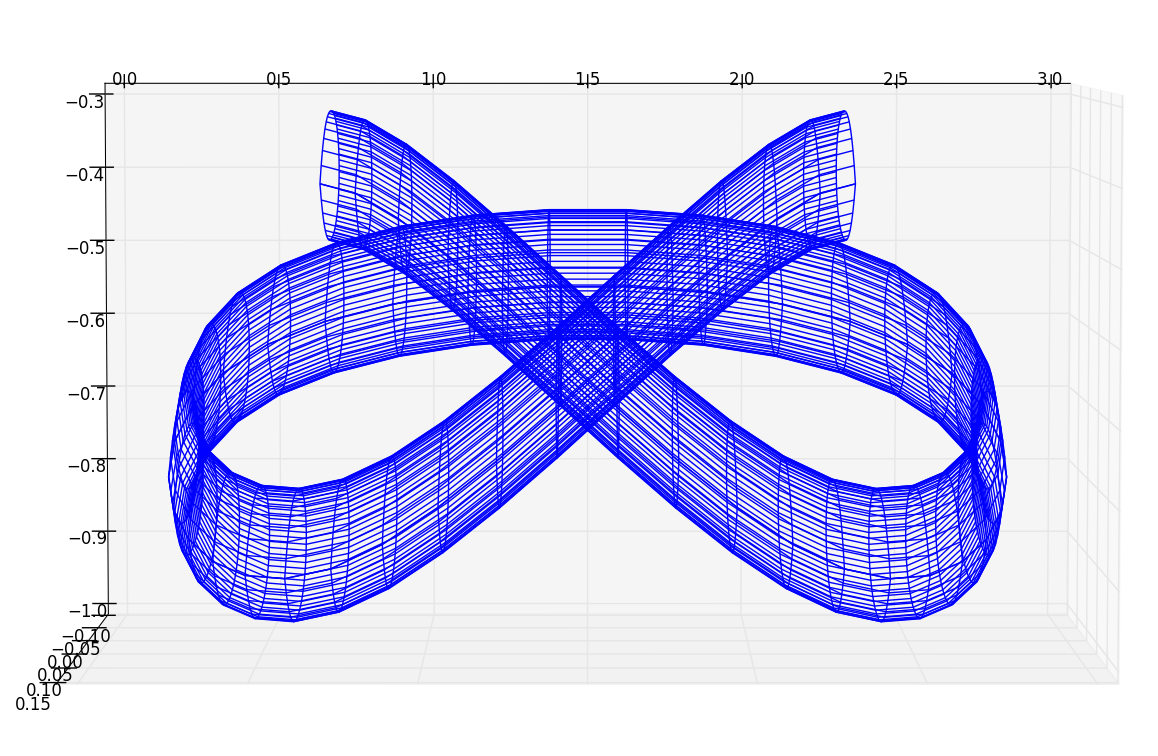
\includegraphics[scale=0.3]{bretzel3d2}
\end{figure}
\begin{figure}[h!]
	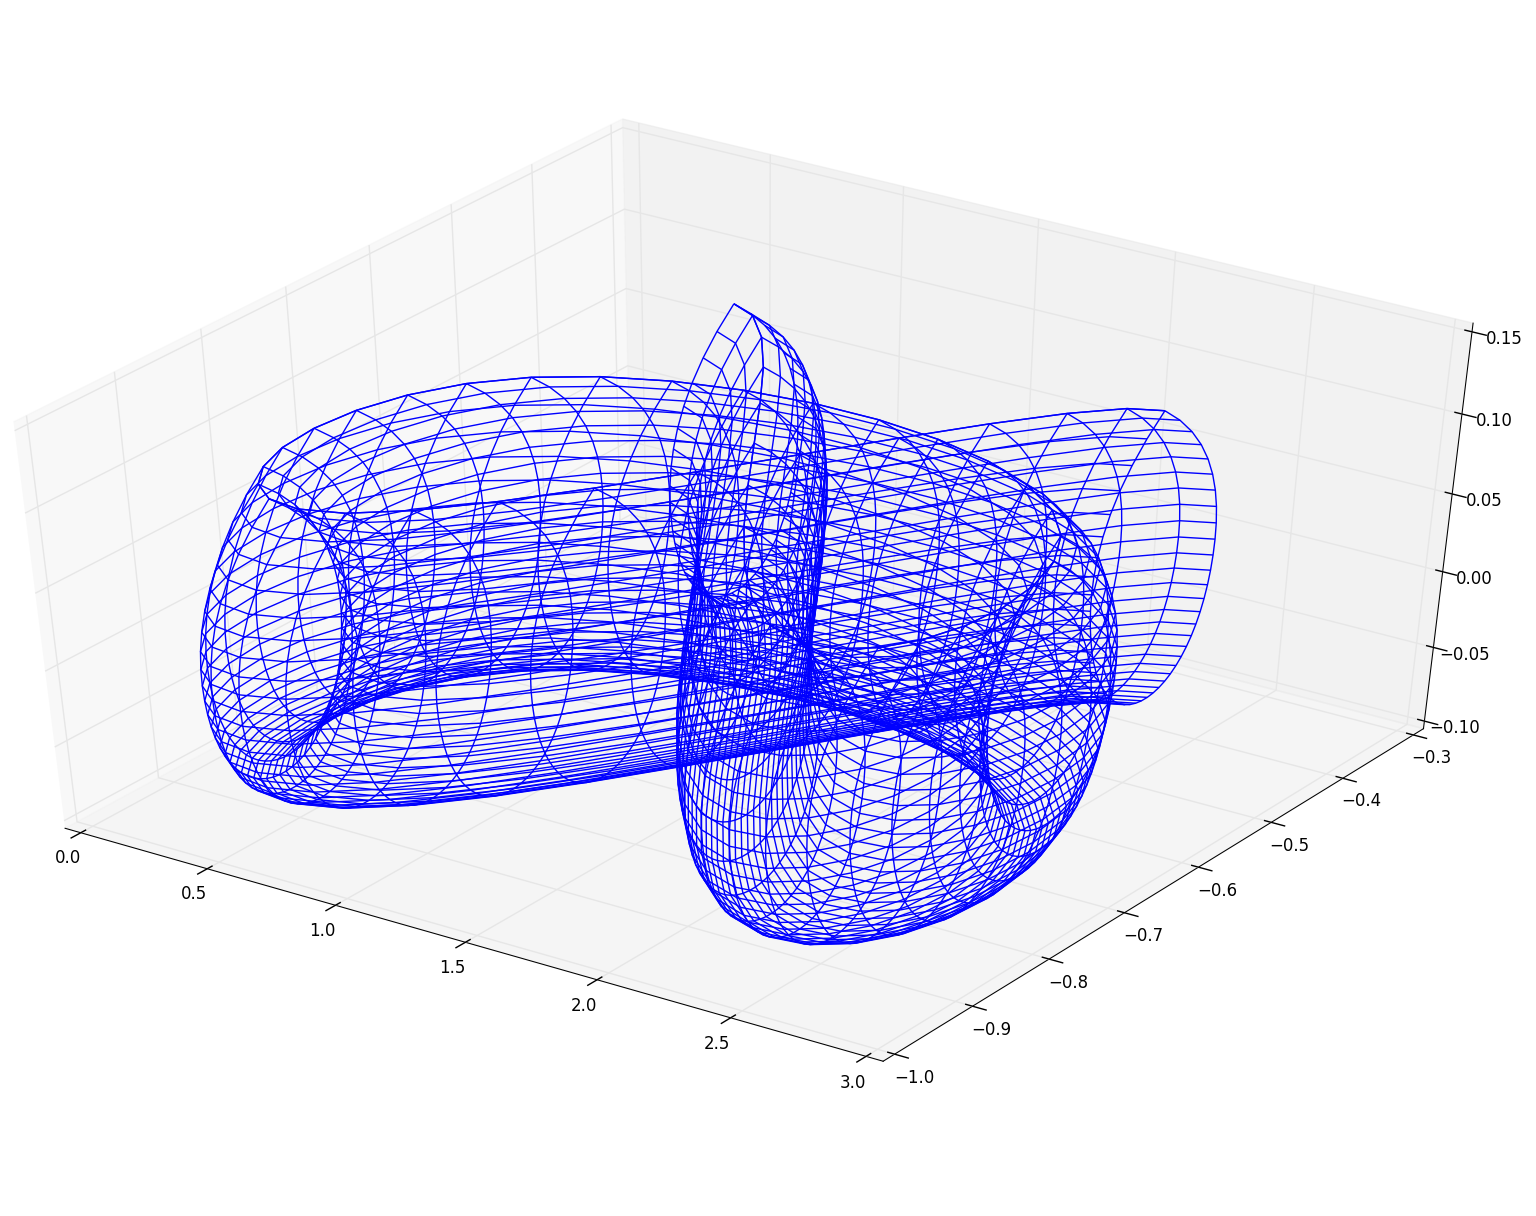
\includegraphics[scale=0.3]{bretzel3d}
\end{figure}
\newpage

\section*{Task 3}
In this task we determine the control points for a planar B\'{e}zier surface to approximate a set of data points. A figure of the surface and its control points, together with the data points can be seen in the figure below and the code can be seen in Appendix I.\\
The control points were determined by first using least squares to determine the coefficients $a, b, c$ of the plane
\begin{equation*}
z = ax + by + c,
\end{equation*}
and the plane was then evaluated at the corners of the minimal rectangle covering the projection of the data points onto the plane in order to obtain the control points.
\begin{figure}[h!]
	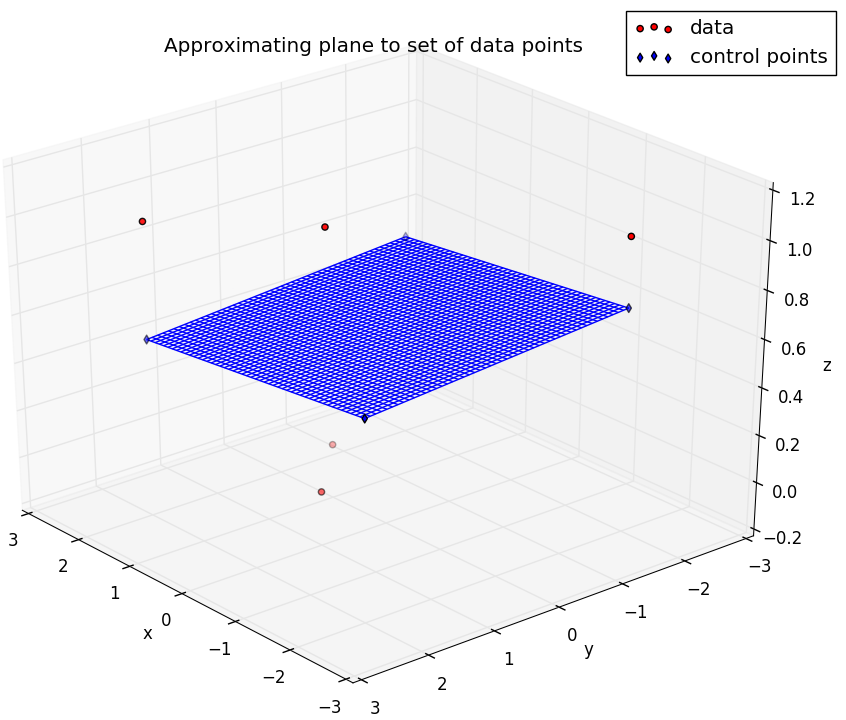
\includegraphics[scale=0.4]{plane}
\end{figure}
\section*{Task 4}
In this task we plot a 3D cone using NURBS. The code can be seen in Appendix I and the figure can be seen below.\\

\begin{figure}[h!]
	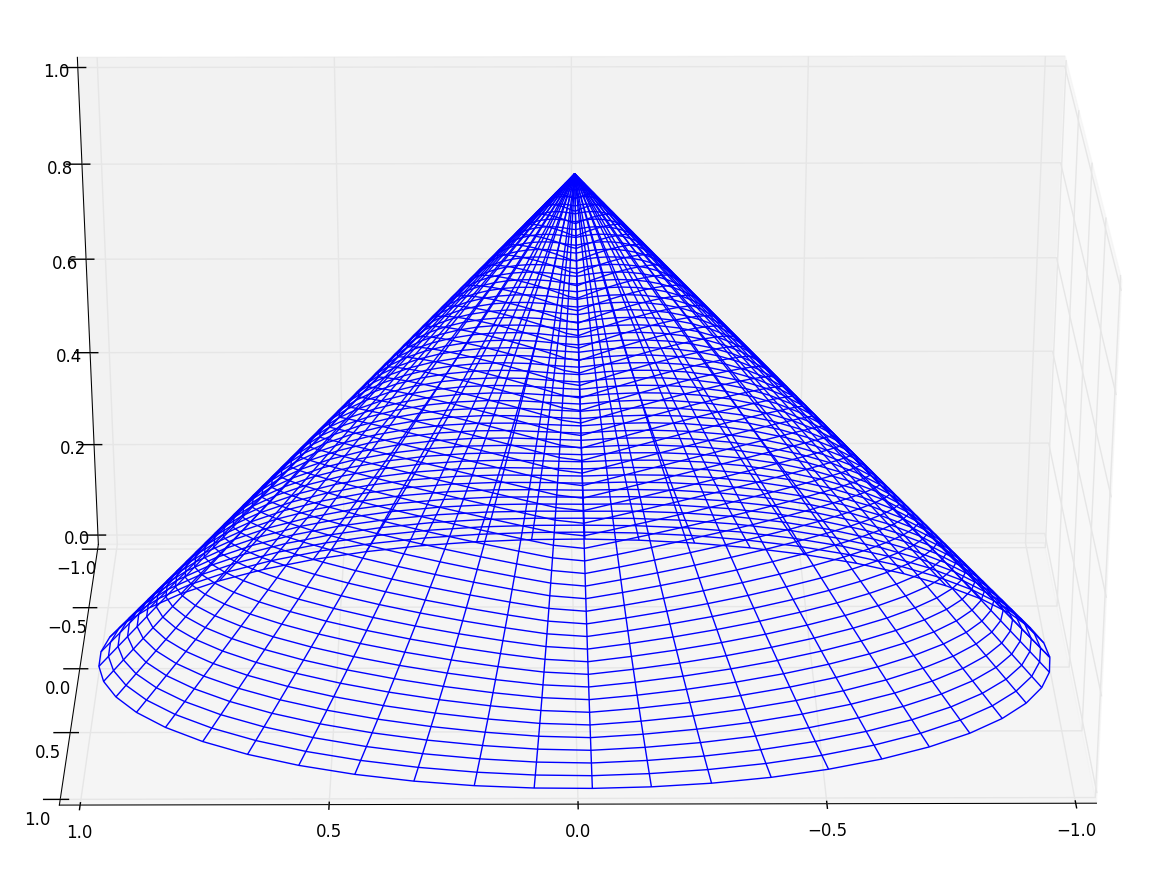
\includegraphics[scale=0.3]{nurbscone}
\end{figure}
\newpage
\section*{Homework 4 task 4 do-over}
In this task we subdivide a 4th degree B-spline into its B\'{e}zier segments. This is done by first subdividing the B-spline at its internal knots into separate B-splines and then constructing B\'{e}zier segments using the control points of these separate B-splines.\\
The B\'{e}zier curves all have the the same degree as the original B-spline, namely 4. The original B-spline and its segments can be seen in the plot below and the code used to construct it can be seen in Appendix I.
\begin{figure}[h!]
	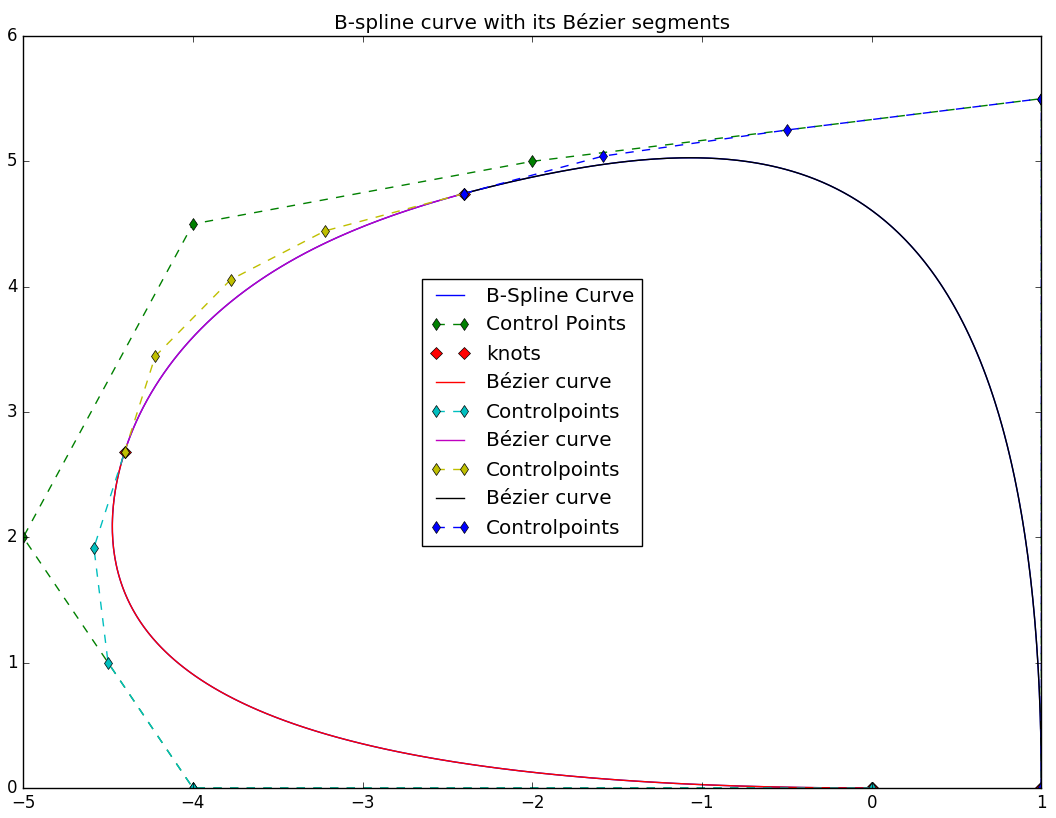
\includegraphics[scale=0.4]{task4_doover}
\end{figure}


\newpage
\section*{Appendix I}
\subsection*{Code for task 1}
\lstinputlisting[firstline=7]{task1.py}

\subsection*{Code for task 3}
\lstinputlisting[firstline=8]{task3.py}

\subsection*{Code for task 4}
\lstinputlisting[firstline=7]{task4.py}

\subsection*{Code for Homework 4 task 4 do-over}
\lstinputlisting[firstline=8]{homework4task4_doover.py}
\end{document}
